\documentclass{article}
\usepackage{graphicx}
\usepackage{amsmath,amsthm,amssymb}
\usepackage[font=small,labelfont=bf]{caption}
\usepackage{tikz}
\usetikzlibrary{calc, angles, quotes, shapes.geometric, decorations.pathreplacing}
\usepackage{tkz-euclide}
\usepackage[inline]{asymptote}
\usepackage{float}
\usepackage[margin=1in]{geometry}
\usepackage{gensymb}
\usepackage[normalem]{ulem}
\usepackage{hyperref}
\hypersetup{
    colorlinks=true,
    linkcolor=blue,
    filecolor=magenta,      
    urlcolor=cyan,
    pdftitle={Overleaf Example},
    pdfpagemode=FullScreen,
    }
\usepackage{fancyhdr}
\pagestyle{fancy}
\fancyhead[R]{Enoch Yu}
\pagenumbering{gobble}
\usepackage{enumitem}
\newtheorem{theorem}{Theorem}[section]
\newtheorem{lemma}[theorem]{Lemma}
\newtheorem*{lemma*}{Lemma}
\newtheorem{sublemma}{Lemma}[section]
\newtheorem{proposition}{Proposition}
\newtheorem{corollary}{Corollary}[theorem]
\newtheorem{example}{Example}[section]
\newtheorem*{example*}{Example}
\newenvironment{solution}{\begin{trivlist}\item[]{\bf Solution}}{\qed \end{trivlist}}
\newcommand{\verteq}{\rotatebox{90}{$\;\;=\;\;$}}
\newcommand*\circled[1]{\tikz[baseline=(char.base)]{
            \node[shape=circle,draw,inner sep=1pt] (char) {#1};}}
\newcommand{\triangled}[1]{\tikz[baseline=(char.base)]{
            \node[shape=regular polygon, regular polygon sides=3, draw, inner sep=0.2pt] (char) {#1};}}

\title{Problem Set 22}
\author{Enoch Yu}
\date{June 2025}

\begin{document}

\section*{2021 Fall AMC 12B Problem 22}
Right triangle $ABC$ has side lengths $BC=6$, $AC=8$, and $AB=10$. A circle centered at $O$ is tangent to line $BC$ at $B$ and passes through $A$. A circle centered at $P$ is tangent to line $AC$ at $A$ and passes through $B$. What is $OP$?
\\\\
$\textbf{(A)}\ \frac{23}{8} \qquad\textbf{(B)}\  \frac{29}{10} \qquad\textbf{(C)}\  \frac{35}{12} \qquad\textbf{(D)}\ \frac{73}{25} \qquad\textbf{(E)}\ 3$
\begin{solution}
\\\\
\textbf{Key Word} Pythagorean Theorem
\\\\
First, the diagram could be drawn. Moreover, finding the distance using Analytic Geometry seems easier.
\begin{center}
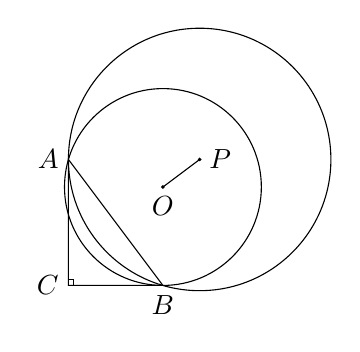
\begin{tikzpicture}[scale=0.2]
    \coordinate (A) at (0,8);
    \coordinate (B) at (6,0);
    \coordinate (C) at (0,0);
    \coordinate (O) at (6,6.25);
    \coordinate (P) at (8.3333,8);
    
    \draw (A) -- (B) -- (C) -- cycle;
    \draw (O) circle (6.2497999968);
    \draw (P) circle (8.3330666624);
    \draw (O) -- (P);

    \node[left] at (A) {$A$};
    \node[below] at (B) {$B$};
    \node[left] at (C) {$C$};
    \node[below] at (O) {$O$};
    \node[right] at (P) {$P$};

    \tkzMarkRightAngle[size=.35](A,C,B);

    \foreach \n in {O, P}
    \node at (\n)[circle,fill,inner sep=0.5pt]{};
\end{tikzpicture}
\end{center}
Using the fact that the circles are tangent to the triangle, the Pythagorean Theorem may be applicable.
The colored triangle may be exploited.
\begin{center}
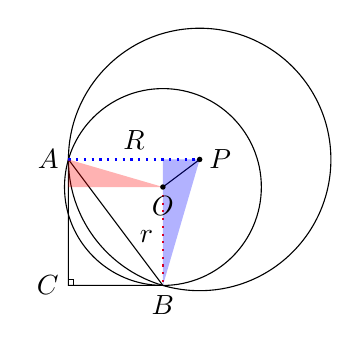
\begin{tikzpicture}[scale=0.2]
    \coordinate (A) at (0,8);
    \coordinate (B) at (6,0);
    \coordinate (C) at (0,0);
    \coordinate (O) at (6,6.25);
    \coordinate (P) at (8.3333,8);
    
    \draw (A) -- (B) -- (C) -- cycle;
    \draw (O) circle (6.2497999968);
    \draw (P) circle (8.3330666624);
    \draw (O) -- (P);

    \draw[red, dotted, thick] (O) -- (B);
    \draw[blue, dotted, thick] (A) -- (P);
    
    \fill[red, opacity=0.3] (O) -- (0, 6.25) -- (A);
    \fill[blue, opacity=0.3] (P) -- (B) -- (6, 8);

    \node[left] at (A) {$A$};
    \node[below] at (B) {$B$};
    \node[left] at (C) {$C$};
    \node[below] at (O) {$O$};
    \node[right] at (P) {$P$};

    \node[left] at ($(O)!0.5!(B)$) {$r$};
    \node[above] at ($(P)!0.5!(A)$) {$R$};

    \tkzMarkRightAngle[size=.35](A,C,B);

    \foreach \n in {O, P}
    \node at (\n)[circle,fill,inner sep=0.7pt]{};
\end{tikzpicture}
\end{center}
Therefore, using the Pythagorean Theorem, $6^2 + (8 - r)^2 = r^2$ and $8^2 + (R - 6)^2 = R^2$ are true.
\begin{align*}
    6^2 + (8 - r)^2 &= r^2 \\
    16r &= 100 \\
    r &= \frac{25}{4}
    \\\\
    8^2 + (R - 6)^2 &= R^2 \\
    12R &= 100 \\
    R &= \frac{25}{3}
\end{align*}
Therefore, using the center of the circles,
\begin{align*}
OP
&= \sqrt{(8 - \frac{25}{4})^2 + (\frac{25}{3} - 6)^2} \\
&= \boxed{\textbf{(C)}\ \frac{35}{12}}.
\end{align*}
\end{solution}

\newpage
\section*{2021 Fall AMC 12B Problem 24}
Triangle $ABC$ has side lengths $AB = 11, BC=24$, and $CA = 20$. The bisector of $\angle{BAC}$ intersects $\overline{BC}$ in point $D$, and intersects the circumcircle of $\triangle{ABC}$ in point $E \ne A$. The circumcircle of $\triangle{BED}$ intersects the line $AB$ in points $B$ and $F \ne B$. What is $CF$?
\\\\
$\textbf{(A) } 28 \qquad \textbf{(B) } 20\sqrt{2} \qquad \textbf{(C) } 30 \qquad \textbf{(D) } 32 \qquad \textbf{(E) } 20\sqrt{3}$
\begin{solution}
\\\\
\textbf{Key Word} Similar Triangle, Power of a Point Theorem, Stewart's Theorem, Law of Cosines \\
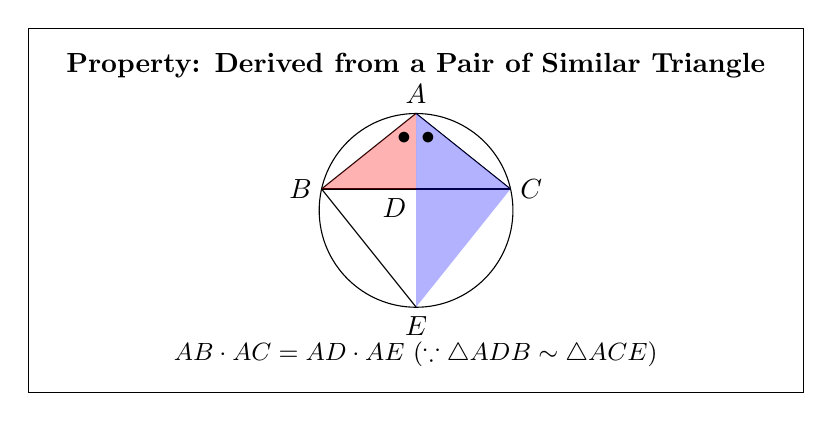
\begin{tikzpicture}[scale=0.4]
    \coordinate (A) at (0, -0.4);
    \coordinate (B) at (3, 2);
    \coordinate (C) at (6, -0.4);
    \coordinate (D) at (3, -0.4);
    \coordinate (E) at (3, -4.15);

    \draw (3, -1.08) circle (3.07571129985);

    \draw (A) -- (B);
    \draw (B) -- (C);
    \draw (C) -- (A);
    \draw (A) -- (E);

    \fill[red, opacity=0.3] (A) -- (B) -- (D);
    \fill[blue, opacity=0.3] (B) -- (C) -- (E);

    \draw pic["$\bullet$", angle eccentricity=0.7] {angle=A--B--D};
    \draw pic["$\bullet$", angle eccentricity=0.7] {angle=D--B--C};

    \node[left] at (A) {$B$};
    \node[above] at (B) {$A$};
    \node[right] at (C) {$C$};
    \node[below left] at (D) {$D$};
    \node[below] at (E) {$E$};

    \coordinate (SW) at (current bounding box.south west);
    \coordinate (NE) at (current bounding box.north east);
    \path[draw=black] 
        ($(SW)+(-8,-1.5)$) rectangle ($(NE)+(8,1.5)$);

    \path let \p1 = ($(SW)+(-3.5,-1)$), \p2 = ($(NE)+(3.5,1)$) in
    coordinate (TopCenter) at ({0.5*(\x1+\x2)}, {\y2})
    coordinate (BottomCenter) at ({0.5*(\x1+\x2)}, {\y1});

    \node[anchor=north, font=\bfseries] at (TopCenter) {Property: Derived from a Pair of Similar Triangle};
    \node[anchor=south, font=\small] at (BottomCenter) {$AB \cdot AC = AD \cdot AE\ (\because \triangle{ADB} \sim \triangle{ACE})$};
\end{tikzpicture}
\\\\
First, the situation could be drawn.
\begin{center}
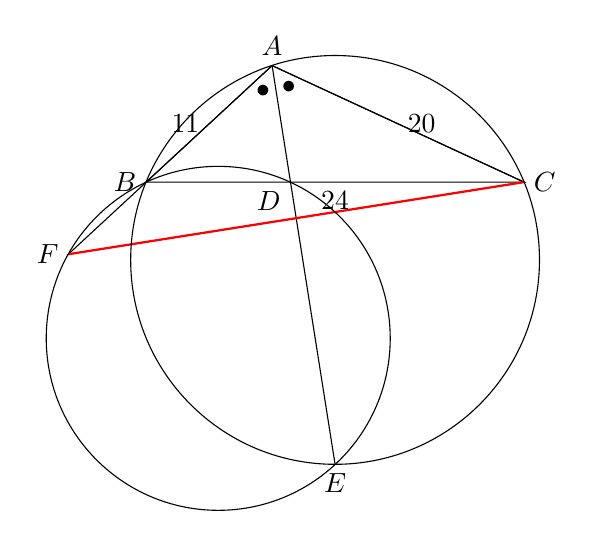
\begin{tikzpicture}[scale=0.4]
    \coordinate (A) at (4, 3.7);
    \coordinate (B) at (0,0);
    \coordinate (C) at (12, 0);
    \coordinate (D) at (4.58, 0);
    \coordinate (E) at (6, -8.96);
    \coordinate (F) at (-2.47, -2.29);

    \draw (A) -- (B) -- (C) -- cycle;
    \draw (A) -- (F) -- (C) -- cycle;
    \draw (A) -- (E);
    \draw[red, thick] (F) -- (C);

    \draw (6, -2.47) circle (6.48999229584);
    \draw (2.29, -4.96) circle (5.46076917659);

    \node[above] at (A) {$A$};
    \node[left] at (B) {$B$};
    \node[right] at (C) {$C$};
    \node[below left] at (D) {$D$};
    \node[below] at (E) {$E$};
    \node[left] at (F) {$F$};
    \node[left] at ($(A)!0.5!(B)$) {$11$};
    \node[right] at ($(A)!0.5!(C)$) {$20$};
    \node[below] at ($(B)!0.5!(C)$) {$24$};

    \draw pic["$\bullet$", angle eccentricity=0.7] {angle=B--A--D};
    \draw pic["$\bullet$", angle eccentricity=0.7] {angle=D--A--C};
\end{tikzpicture}
\end{center}
Using the similar triangle, notice that $AD \cdot AE = 11 \cdot 20$. Moreover, using the Power of a Point Theorem, it is evident that $AF = 20$. Two possible pathways are resulted.
\\\\
\begin{minipage}{0.48\textwidth}
\textbf{Stewart's Theorem}
\begin{align*}
    11 \cdot FC^2 + 9 \cdot 20^2 &= (11 + 9)(11 \cdot 9 + 24^2) \\
    11FC^2 + 3600 &= (20)(99 + 576) \\
    11FC^2 + 3600 &= 20 \cdot 675 \\
    11FC^2 &= 9900 \\
    \therefore FC = \boxed{\textbf{(C) } 30}
\end{align*}
\end{minipage}
\hfill
\begin{minipage}{0.48\textwidth}
\textbf{Law of Cosines}
\begin{align*}
    \frac{11^2 + 20^2 - 24^2}{2 \cdot 11 \cdot 20} &= \frac{20^2 + 20^2 - FC^2}{2 \cdot 20 \cdot 20} \\
    -5 &= \frac{800 - FC^2}{20} \\
    -100 &= 800 - FC^2 \\
    \therefore FC = \boxed{\textbf{(C) } 30}
\end{align*}
\end{minipage}
\end{solution}

\newpage
\section*{Problem}
Compute the smallest positive angle $x$, in degrees, such that $\tan4x = \frac{\cos{x} - \sin{x}}{\cos{x} + \sin{x}}$.
\begin{solution}
\\\\
\textbf{Key Word} Trigonometric Identities
\\\\
\begin{align*}
    \frac{\sin4x}{\cos4x} &= \frac{\cos{x} - \sin{x}}{\cos{x} + \sin{x}} \\
    \sin4x \cdot \cos{x} + \sin4x \dot \sin{x} &= \cos{x} \cdot \cos4x - \sin{x} \cdot \cos4x \\
    \sin4x \cdot \cos{x} + \sin{x} \cdot \cos4x &= \cos{x} \cdot \cos4x - \sin4x \dot \sin{x} \\
    \sin(x + 4x) &= \cos(x + 4x) \\
    \sin5x &= \cos 5x \\
    \therefore x \Rightarrow \boxed{9^{\circ}}
\end{align*}
\end{solution}

\section*{Problem}
Prove that for all real $x$ and $y$, we have $-\frac{1}{2} \le \frac{(x + y)(1 - xy)}{(1 + x^2)(1 + y^2)} \le \frac{1}{2}$.
\begin{proof}
    Let $x = \tan\alpha$ and $y = \tan\beta$.
    \begin{align*}
        \frac{(\tan\alpha + \tan\beta)(1 - \tan\alpha \cdot \tan\beta)}{(1 + \tan^2\alpha)(1 + \tan^2\beta)}
        &= \frac{(\tan\alpha + \tan\beta)(1 - \tan\alpha \cdot \tan\beta)}{\sec^2\alpha \cdot \sec^2\beta} \\[0.7em]
        &= \left( \frac{\sin\alpha}{\cos\alpha} + \frac{\sin\beta}{\cos\beta} \right) \left( 1 - \frac{\sin\alpha \cdot \sin\beta}{\cos\alpha \cdot \cos\beta} \right) (\cos^2\alpha \cdot \cos^2\beta) \\[0.7em]
        &= (\sin\alpha\cos\beta + \sin\beta\cos\alpha)(\cos\alpha\cos\beta - \sin\alpha\sin\beta) \\[0.7em]
        &= \sin(\alpha + \beta)\cos(\alpha + \beta) \\[0.7em]
        &= \frac{1}{2}\sin(2(\alpha + \beta))
        \\\\
        -\frac{1}{2} \le &\frac{1}{2}\sin(2(\alpha + \beta)) \le \frac{1}{2} \\
        \therefore -\frac{1}{2} \le &\frac{(x + y)(1 - xy)}{(1 + x^2)(1 + y^2)} \le \frac{1}{2}
    \end{align*}
\end{proof}

\newpage
\section*{Problem}
Determine all $\theta$ such that $0 \le \theta \le \frac{\pi}{2}$ and $\sin^5\theta + \cos^5\theta = 1$.
\begin{solution}
\\\\
\textbf{Key Word}
\\\\
For $|r| < 1$, 
\[
\lim_{n \rightarrow \infty}{|r|^n} = 0.
\]
Moreover, $-1 \le |\sin\theta||\cos\theta| \le 1$. Using the first fact, the following inequalities and equations are true.
\begin{align*}
\cos^2\theta &\ge \cos^5\theta \\
\sin^2\theta &\ge \cos^5\theta
\\\\
\sin^2\theta + \cos^2\theta &= 1 \\
\sin^5\theta + \cos^5\theta &= 1
\end{align*}
In order to satisfy the given conditions, $\sin^2\theta = \sin^5\theta$ and $\cos^2\theta = \cos^5\theta$ must be true.
\begin{align*}
    1 &= \sin^3 \qquad \text{Unless 0} \\
    1 &= \cos^3 \qquad \text{Unless 0}
\end{align*}
Therefore, $\theta = \boxed{0, \frac{\pi}{2}}$
\end{solution}

\section*{Problem}
Suppose that $\sec\theta + \tan\theta = \frac{22}{7}$. Find $\csc\theta + \cot\theta$.
\begin{solution}
\\\\
\textbf{Key Word} \textcolor{red}{MUST THINK OF THIS WHEN YOU SEE $\sec\theta + \tan\theta$!!} \\
\begin{minipage}{0.48\textwidth}
\begin{align*}
    \sin^2\theta + \cos^2\theta &= 1 \\
    1 + \cot^2\theta &= \csc^2\theta \\
    \tan^2\theta + 1 &= \sec^2\theta
\end{align*}
\end{minipage}
\begin{minipage}{0.48\textwidth}
\begin{align*}
    (\csc\theta + \cot\theta)(\csc\theta - \cot\theta) &= 1 \\
    (\sec\theta + \tan\theta)(\sec\theta - \tan\theta) &= 1 \\
    \sec\theta + \tan\theta = \frac{22}{7},\ \sec\theta - \tan\theta &= \frac{7}{22}
\end{align*}
\end{minipage} \\
\begin{minipage}{0.48\textwidth}
\begin{align*}
    2\sec\theta &= \frac{533}{154} \\
    \therefore \sec\theta &= \frac{533}{308}
    \\\\
    2\tan\theta &= \frac{435}{154} \\
    \therefore \tan\theta &= \frac{435}{308} \\
    \therefore \cot\theta &= \frac{1}{\frac{435}{308}}  \\
    &= \frac{308}{435}
\end{align*}
\end{minipage}
\begin{minipage}{0.48\textwidth}
\begin{align*}
    \sin\theta
    &= \frac{\tan\theta}{\sec\theta} \\
    &= \frac{435}{533} \\
    \therefore \csc\theta &= \frac{533}{435}
    \\\\
    \therefore \csc\theta + \cot\theta
    &= \frac{533}{435} + \frac{308}{435} \\
    &= \frac{841}{435} \\
    &= \boxed{\frac{29}{15}}
\end{align*}
\end{minipage}

\end{solution}

\end{document}
